\documentclass{standalone}
\usepackage{pgfplots}
\pgfplotsset{compat=1.18} % Adjust version if needed

\begin{document}
	
	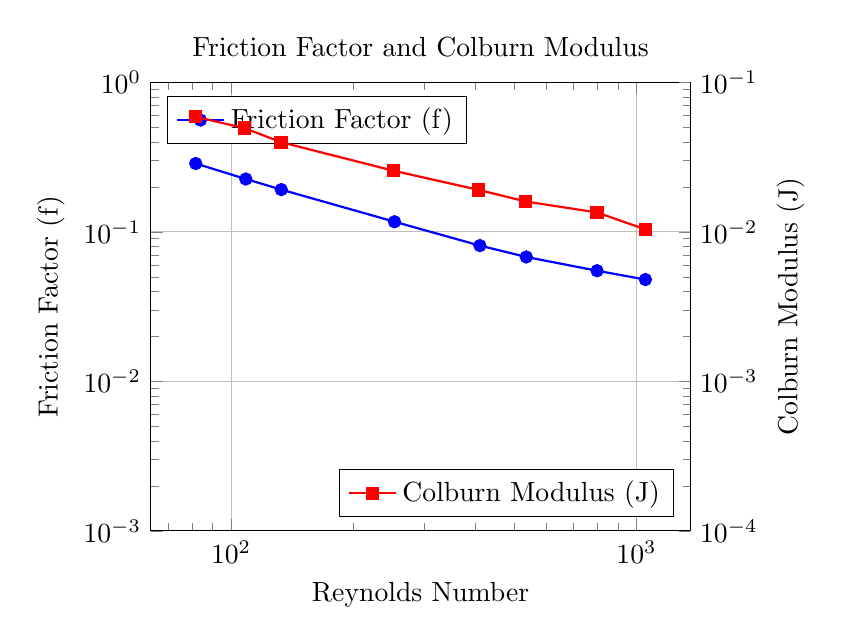
\begin{tikzpicture}
		\begin{loglogaxis}[
			xlabel={Reynolds Number},
			ylabel={Friction Factor (f)},
			grid=major,
			title={Friction Factor and Colburn Modulus},
			legend entries={Friction Factor (f)},
			legend pos=north west,
			axis y line*=left, % Left y-axis for f
			ymin=0.001, ymax=1, % Adjust y-range for f
			]
			% Sample data for Friction Factor (f)
			\addplot[
			color=blue,
			mark=*,
			thick
			] coordinates {
(81.8, 0.287)
(108.7, 0.226)
(133, 0.192)
(253, 0.117)
(410.9, 0.081)
(534.7, 0.068)
(799.4, 0.055)
(1052, 0.048)
			};
		\end{loglogaxis}
		
		\begin{loglogaxis}[
			ylabel={Colburn Modulus (J)},
			axis y line*=right, % Right y-axis for J
			axis x line=none,   % Hide duplicate x-axis
			ymin=0.0001, ymax=0.1, % Adjust y-range for J
			legend entries={Colburn Modulus (J)},
			legend pos=south east,
			]
			% Sample data for Colburn Modulus (J)
			\addplot[
			color=red,
			mark=square*, % Different marker for distinction
			thick
			] coordinates {
(80.5, 0.0589)
(106.3, 0.0495)
(130.8, 0.0399)
(247.9, 0.0257)
(403.3, 0.0191)
(526.1, 0.016)
(790.9, 0.0135)
(1041.8, 0.0104)
			};
		\end{loglogaxis}
	\end{tikzpicture}
	
\end{document}